% \documentclass[a4paper,landscape,columns=2]{cheatsheet}
\documentclass[10pt, a4paper]{article}

\usepackage{geometry}

\input{mymathpreamble.tex}

\usepackage{mathtools}

% giving this a try:
% http://www.khirevich.com/latex/microtype/
\usepackage[activate={true,nocompatibility},final,tracking=true,kerning=true,spacing=true,factor=1100,stretch=10,shrink=10]{microtype}

\usepackage{pdflscape}

\usepackage{multicol}
\setlength{\columnsep}{0.8cm}

\usepackage{wrapfig}

\usepackage{titlesec}
\titleformat*{\section}{\large\bfseries}
\titlespacing*{\section}{0pt}{2ex}{2ex}  % 4.3ex plus .2ex

\usepackage{tabularx}
\usepackage{booktabs}
\usepackage{tcolorbox}
\usepackage{enumitem}

\usepackage{tikz}
\usepackage{tikzducks}

\usepackage[style=ieee]{biblatex}
\addbibresource{bibliography.bib}

\usepackage{hyperref}
\usepackage{cleveref}

% https://tex.stackexchange.com/a/51349
\hypersetup{
  colorlinks = true,
  urlcolor = blue,
  linkcolor = blue,
  citecolor = red
}

\setcounter{secnumdepth}{0}  % get rid of section numbering - no need to use \section*

% https://tex.stackexchange.com/a/390653
\newlength{\interwordspace}
\settowidth{\interwordspace}{\ }

\pagenumbering{gobble}

\begin{document}

% \setlength{\abovedisplayskip}{0pt}
% \setlength{\belowdisplayskip}{0pt}
% \setlength{\abovedisplayshortskip}{0pt}
% \setlength{\belowdisplayshortskip}{0pt}

\newgeometry{margin=10mm}

\begin{landscape}
\begin{multicols}{2}
    \raggedcolumns

    \section{Coupled ODEs}

    \[\dot{\vec{y}} = \mat{A} \vec{y} + \vec{r}\]
    %
    \[
        \ddot y + p(t) y + q(t) = r(t) \longrightarrow
        \begin{pmatrix}
            y \\
            \dot y
        \end{pmatrix}
        = \dot{\vec{y}} = \begin{pmatrix}
            0 & 1 \\
            -q(t) & -p(t)
        \end{pmatrix} \vec{y} + \begin{pmatrix}
            0 \\
            r(t)
        \end{pmatrix}
    \]

    The eigenvalues of \(\mat{A}\) found by solving \(\det (\mat{A} - \lambda \mat{I}) = 0\)
    gives the same characteristic equation for the uncoupled system. General solutions for
    a second-order system with real constant coefficients, with
    eigenvalues \(\lambda_1, \lambda_2\) and eigenvectors \(\vec{x_1}, \vec{x_2}\), are given by:
    \begin{align*}
        \lambda_1 \neq \lambda_2: \enspace
            \vec{y} &= c_1 \vec{x_1} e^{\lambda_1 t} + c_2 \vec{x_2} e^{\lambda t} \\
        \lambda_1, \lambda_2 \in \mathbb{C}: \enspace
            \vec{y} &= c_1 \Re\left(\vec{x_1} e^{\lambda_1 t}\right) 
                + c_2 \Im\left(\vec{x_1} e^{\lambda_1 t}\right) \\
        \lambda_1 = \lambda_2: \enspace
            \vec{y} &= c_1 \vec{x} e^{\lambda t} + c_2 (t \vec{x} + \vec{p}) e^{\lambda t},
            \,\text{where}\, (\mat{A} - \lambda \mat{I}) \vec{p} = \vec{x}.
    \end{align*}

    \section{Phase Portraits of 2D Autonomous Systems}

    Let \(\dot{\vec{y}} = \vec{f}(\vec{y})\) with \(\vec{y} \in \mathbb{R}^2\),
    \(\vec{f}: \mathbb{R}^2 \to \mathbb{R}^2\), where \(\vec{f}\) does not depend on \(t\).
    \(\vec{f}\) defines a direction field in
    the \(y_1\)-\(y_2\) plane, and a \emph{trajectory} of the system is a curve following the
    field. \(\vec{f}\) being continuous with continuous partials implies existence and uniqueness
    for these trajectories, so they do not cross. By the chain rule, the slope of a trajectory is
    \[\oderiv{y_2}{y_1} = \frac{\dot y_2}{\dot y_1} = \frac{f_2}{f_1}.\]
    %
    A \emph{nullcline} is a curve in phase space where the slope of the trajectory is either 0 or \(\infty\).
    Set \(\dot y_2 = 0\) for horizontal nullclines and \(\dot y_1 = 0\) for vertical nullclines, and
    solve for \(y_2\). Solving for the trajectories themselves is possible in specific cases,
    usually when the ODE in \(y_2\) from the slope formula is separable.

    For the lines in phase space in the direction of the eigenvectors (called \emph{eigendirections}),
    there are straight line solutions either flowing towards or away from the origin, determined
    by the sign of the corresponding eigenvalue (\(-\) stable, \(+\) unstable).
    
    \(\lambda_1 \neq \lambda_2\) and both have the same sign:
    \begin{itemize}
        \item Negative \(\lambda\) gives a \emph{stable improper node}, where
            trajectories curve like a parabola and approach the eigendirection with smallest absolute value,
            since that exponential term dominates at large \(t\).
        \item Positive \(\lambda\) gives an
            \emph{unstable improper node}, where trajectories approach eigendirection with
            largest absolute value.
    \end{itemize}

    \(\lambda_1 > 0,\, \lambda_2 < 0\):
    \begin{itemize}
        \item This gives a \emph{saddle point}. Trajectories come in parallel to the
            stable eigendirection then turn around and become parallel to the unstable direction.
    \end{itemize}
    %
    \vfill\columnbreak
    %
    \(\lambda_1 = \lambda_2\):
    \begin{itemize}
        \item If there are 2 linearly independent eigenvectors (eigenspace of \(\lambda\) has dimension 2),
            all trajectories travel in straight lines either towards or away from the origin, called
            a \emph{proper node}. For a 2D system, this is only possible if \(\mat{A}\) is some multiple of
            the identity matrix, i.e. \(\mat{A} = k \mat{I}\) for \(k \in \mathbb{R}\).
        \item If there is only 1 eigenvector, trajectories come tangent to the eigendirection near the origin
            and do a U-turn away, called a \emph{degenerate node}.
    \end{itemize}

    \(\lambda = \alpha \pm \beta i\):
    \begin{itemize}
        \item If \(\alpha = 0\), trajectories are ellipses around the origin, and the origin
            is called a \emph{centre}. To determine the direction of flow, consider the sign of \(\dot y_1\)
            at a point in the positive quadrant.
        \item If \(\alpha \neq 0\), trajectories trace out a logarithmic spiral \(r(t) = e^{\alpha t}\)
            shown by converting to polar coordinates. This is called a \emph{spiral}.
            Plotting nullclines helps with sketching trajectories.
    \end{itemize}

    The following stability chart allows for the system to be classified given values of
    \(\tr \mat{A}\) and \(\det \mat{A}\) \cite{StabilityDiagram}. The discriminant
    \(\Delta\) is defined as \(\Delta = (\tr \mat{A})^2 - 4 \det \mat{A}\).

    {%
        \centering
        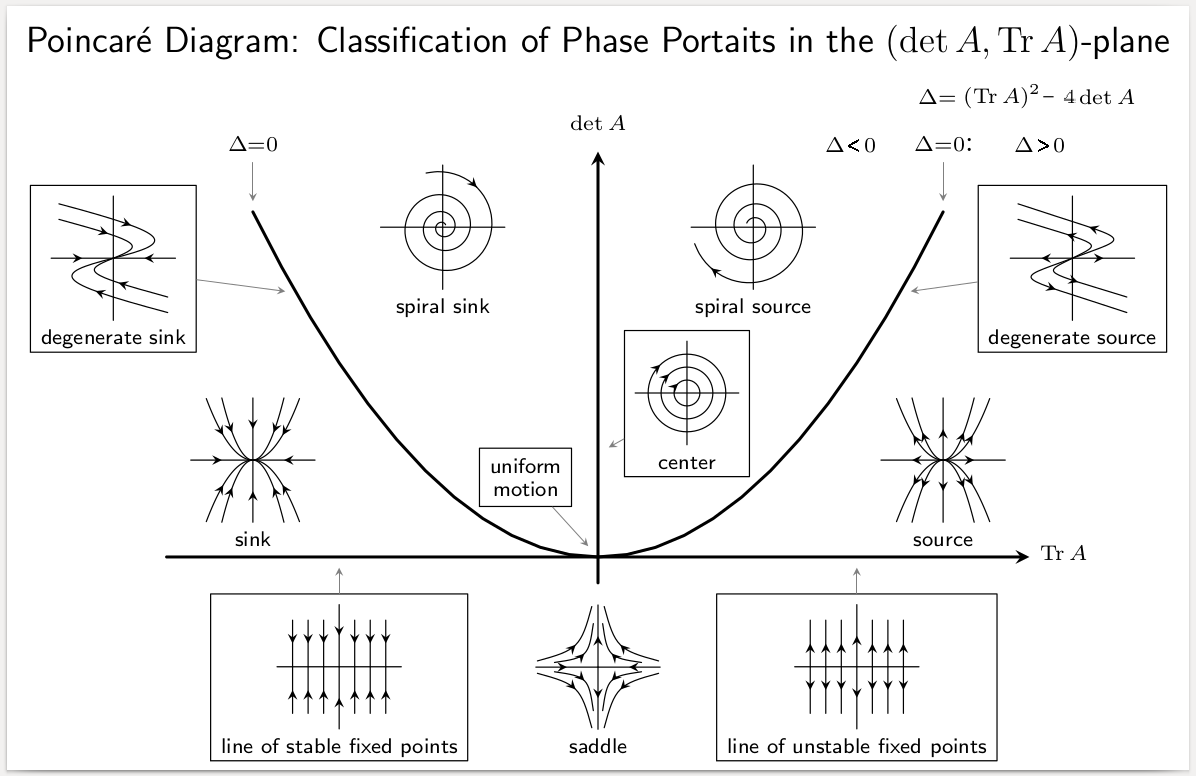
\includegraphics[width=\columnwidth]{images/stabilityDiagram.png}
    }%

    \begin{tcolorbox}[colframe=red!75!black, arc=0pt, outer arc=0pt, center, hbox]
        ducky's MATH2100 summary --- \today
    \end{tcolorbox}

\end{multicols}

\pagebreak

\begin{multicols}{2}
    \section{Non-Linear or Inhomogeneous Systems}

    A system \(\dot{\vec{y}} = \vec{f}(\vec{y})\) has a \emph{critical point} at \(\vec{y^*}\) if
    \(\vec{f}(\vec{y^*}) = \vec{0}\). Linear systems always have one at \(\vec{0}\), and only one
    unless \(\det \mat{A} = 0\).
    %
    An inhomogeneous linear system \(\dot{\vec{y}} = \mat{A}\vec{y} + \vec{p}\) is a linear
    translation away from a homogeneous system. Shifting the critical point at \(\vec{p}\) to
    \(\vec{0}\) via the change of variables \(\vec{x} = \vec{y} - \vec{p}\) gives the homogeneous
    \(\dot{\vec{x}} = \mat{A} \vec{x}\), so techniques discussed earlier are applicable.
    
    For a nonlinear system \(\dot{\vec{y}} = \vec{f}(\vec{y})\), the nature of the system around the
    critical point is approximated via the \emph{Jacobian matrix} \(\mat{D}\vec{f}\). 
    The stability diagram can be used to classify these critical points by evaluating \(\mat{D}\vec{f}\)
    at each \(\vec{y^*}\). The \emph{linearised system} near \(\vec{y^*}\) is then
    \[
        \dot{\vec{y}} = \mat{D}\vec{f} |_{\vec{y^{*}}} (\vec{y} - \vec{y^*}),
        \quad
        \mat{D}\vec{f} = \begin{pmatrix}
            \pderiv{f_1}{y_1} & \pderiv{f_1}{y_2} \\
            \pderiv{f_2}{y_1} & \pderiv{f_2}{y_2}
        \end{pmatrix}.
    \]
    %
    \section{Special Functions}

    The \emph{Dirac Delta function} \(\delta(t)\) is an ``impulse'' with infinite value at \(t = 0\) and
    zero value everywhere else, satisfying \(\int_0^{\infty} \delta(t) = 1\). \(\delta(t - a)\)
    represents an impulse at \(t = a\).

    The \emph{unit step function} \(u(t)\) is defined by
    \[
        u(t) = \begin{cases}
            0, & t < 0 \\
            1, & t \geq 0.
        \end{cases}  
    \]
    To write a piecewise-continuous function in terms of \(u\),
    if \(f(t)\) changes from \(g_1(t)\) to \(g_2(t)\) at \(t = c\), add a \(u(t-c) (g_2(t) - g_1(t))\) term
    to the new expression of \(f\) \cite{LaplacePractice}.

    The \emph{Gamma function} \(\Gamma(z)\) generalises the factorial by
    \(\Gamma(n + 1) = n!\) for \(n \in \mathbb{N}\), and is defined for all positive \(z\) by
    \[
        \Gamma(z) = \int_0^{\infty} e^{-x} x^{z-1} \,\deriv x,
    \]

    In this course the \emph{error function} is defined as
    \[
        \erf(x) = \frac{2}{\sqrt{\pi}} \int_0^x e^{-u^2} \,\deriv u.
    \]
    It is odd and monotone increasing. The following formulas may be useful for computation:
    \[
        \int_0^{\infty} e^{-u^2} \,\deriv u = \int_{-\infty}^{0} e^{-u^2} \,\deriv u
        = \frac{\sqrt{\pi}}{2},
        \quad
        \frac{1}{\sqrt{\pi}} \int_a^b e^{-u^2} \,\deriv u
        = \erf(b) - \erf(a).
    \]

    For the heat equation with parameter \(c\), the \emph{Gaussian function} \(G(x, t)\) is defined as
    \[
        G(x, t) = \frac{1}{\sqrt{4 \pi c^2 t}} \exp \left(
            \frac{-x^2}{4c^2 t}
        \right).
    \]
    \(\int_{-\infty}^{\infty} G(x, t) \,\deriv x = 1\) for \(t > 0\),
    \(\lim_{t \to 0^+} G(x, t) = 0\) for \(x \neq 0\) and
    \(\lim_{t \to 0^+} G(0, t) = +\infty\).

    \section{Laplace Transforms}

    The following formulas are given in the formula sheet for the exam, but have been
    added here for completeness.
    \[
        \laplace\{f(t)\} = F(s) = \int_0^{\infty} f(t) e^{-st} \,\deriv t
    \]

    {
    \everymath{\displaystyle}
    % \renewcommand{\arraystretch}{2}
    \begin{center}
    \begin{tabular}{cc@{\hskip 1cm}cc}
        \toprule
        \(f(t)\) & \(F(s)\) & \(f(t)\) & \(F(s)\) \\
        \midrule \\[-10pt]
        \(c\) & \(\frac{c}{s}\) & \(a g(t) + b h(t)\) & \(a G(s) + b H(s)\) \\[10pt]
        \(t^{n}\) & \(\frac{n!}{s^{n+1}}\) & \(e^{at} f(t)\) & \(F(s-a)\) \\[10pt]
        \(t^{a}\) & \(\frac{\Gamma(a+1)}{s^{a+1}}\) & \(f(t-k)u(t-k)\) & \(e^{-ks} F(s)\) \\[10pt]
        \(\cos \alpha t\) & \(\frac{s}{s^{2} + \alpha^{2}}\) & \(f'(t)\) & \(s F(s) - f(0)\) \\[10pt]
        \(\sin \alpha t\) & \(\frac{\alpha}{s^{2} + \alpha^{2}}\) & \(f''(t)\) & \(s^{2} F(s) - sf(0) - f'(0)\) \\[10pt]
        \(\delta(t - k)\) & \(e^{-ks}\) & \(t f(t)\) & \(-F'(s)\) \\[1pt]
        \bottomrule
    \end{tabular}
    \end{center}
    }

    The convolution theorem states that:
    \[
        \laplace^{-1} \left\{F(s) G(s)\right\}
        = \int_0^t f(\tau) g(t - \tau) \,\deriv \tau
        = (f * g)(t).
    \]
    If \(f(t)\) has period \(p\), then the Laplace integral can be simplified:
    \[
        \laplace\{f(t)\}
        = \frac{1}{1 - e^{-sp}} \int_0^p f(t) e^{-st} \,\deriv t.
    \]
    %
    The following formulas are not included in the formula sheet, but may be helpful to know.
    \begin{align*}
        \laplace^{-1} \left\{\frac{s}{(s^2 + \alpha^2)^2}\right\} &= \frac{1}{2\alpha} t \sin \alpha t \\
        \laplace \{f(t) u(t-k)\} &= e^{-ks} \laplace\{f(t+k)\} \tag*{\cite{LaplacePractice}} \\
        \laplace \{f^{(n)}(t)\} &= s^n F(s) - \sum_{k=1}^n s^{n-k} f^{(k-1)}(0) \\
        \laplace \{t^n f(t)\} &= (-1)^n F^{(n)}(s).
    \end{align*}

\end{multicols}


\pagebreak

% \newgeometry{left=10mm,right=10mm,top=15mm,bottom=15mm}
% \vspace*{\fill}
% \onecolumn

% \vspace{-0.5cm}
\begin{multicols}{2}
    \section{Differential Operators and Change of Variables}

    A homogeneous linear differential equation has the form \(L(u) = 0\) where \(L\) is a
    \emph{linear differential operator} satisfying \(L(u+v) = L(u) + L(v)\) and
    \(L(cu) = c L(u)\) for \(c \in \mathbb{R}\) and functions \(u, v\). This can be used
    to verify a DE is linear using the linearity of the derivative. A common differential operator
    is the \emph{del} operator \(\grad\), defined in 3 dimensions by
    \(\grad = (\pderiv{}{x}, \pderiv{}{y}, \pderiv{}{z})\). It can be applied to a scalar field
    \(f\) to get \(f\)'s \emph{gradient field}, or be dotted or crossed with a vector field \(\vec{v}\)
    to get its \emph{divergence} or \emph{curl}:
    \begin{gather*}
        \operatorname{grad} f = \grad f = \left(\pderiv{f}{x}, \pderiv{f}{y}, \pderiv{f}{z}\right),
        \qquad
        \div \vec{v} = \grad \cdot \vec{v} = \pfrac{v_1}{x} + \pfrac{v_2}{y} + \pfrac{v_3}{z}, \\
        \curl \vec{v} = \grad \times \vec{v} = 
        \begin{vmatrix}
            \uvec{i} & \uvec{j} & \uvec{k} \\
            \pfrac{}{x} & \pfrac{}{y} & \pfrac{}{z} \\
            v_1 & v_2 & v_3
        \end{vmatrix}.
    \end{gather*}
    Additionally, the \emph{Laplacian} is defined as \(\grad^2 = \grad \cdot \grad\). For scalar fields,
    \[
        \grad^2 f = \grad \cdot \grad f = \pderiv[2]{f}{x} + \pderiv[2]{f}{y} + \pderiv[2]{f}{z},
    \]
    and for a vector field \(\vec{v}\) in cartesian coordinates, the Laplacian is just defined
    elementwise, so \(\grad^2 \vec{v} = (\grad^2 v_1, \grad^2 v_2, \grad^2 v_3)\).
    Equivalently, it can be defined as
    \[
        \grad^2 \vec{v} = \grad(\grad \cdot \vec{v}) - \grad \times (\grad \times \vec{v}).
    \]
    The above formulas only apply for cartesian coordinates; other coordinate systems have
    different expressions. Importantly, the Laplacian in polar coordinates is given by
    \[
        \grad^2 = \frac{1}{r} \pderiv{}{r} \left(r \pderiv{}{r}\right) + \frac{1}{r^2} \pderiv[2]{}{\theta}.
    \]
    Changing variables that a PDE is expressed in may simplify the equation and give different
    types of solutions not apparent from the initial coordinate system.
    The goal is to express derivatives in the \emph{initial} coordinates in terms of
    derivatives in the \emph{new} coordinates. If \(f(x, y)\) is changed to \(f(u, v)\) via
    \(u(x, y)\) and \(v(x, y)\), then by the chain rule,
    \begin{align*}
        \pderiv{f}{x} &= \pderiv{f}{u} \pderiv{u}{x} + \pderiv{f}{v} \pderiv{v}{x}, \\
        \pderiv{f}{y} &= \pderiv{f}{u} \pderiv{u}{y} + \pderiv{f}{v} \pderiv{v}{y}.
    \end{align*}
    Note that \(f\) can be removed from the above equations to get a relationship purely involving
    the differential operators \(\pderiv{}{x}, \pderiv{}{y}, \pderiv{}{u}\) and \(\pderiv{}{v}\).
    This can then be substituted into the original PDE to get a new equation.

    An example is with the PDE \(u_t + c u_x = 0\) for \(u(x, t)\). Changing variables to
    \(x' = x - ct\) and \(t' = t\) allows the equation to be written as \(u_{t'} = 0\), thus
    \(u(x', t') = f(x')\) and \(u(x, t) = f(x-ct)\) for differentiable \(f\). The solution is
    defined on a plane in \(x\)-\(t\) space.
    
    \section{Fourier Series}

    If a function \(f(x)\) has period \(2L\), i.e. \(f(x + 2L) = f(x)\) for all \(x\), then
    it can be written as a \emph{Fourier series}:
    \[
        f(x)
        = a_0 + \sum_{n=1}^{\infty} \left(
            a_n \cos\left(\frac{n \pi x}{L}\right)
            + b_n \sin\left(\frac{n \pi x}{L}\right)
        \right),
    \]
    with Fourier coefficients given by
    \begin{gather*}
        a_n = \frac{1}{L} \int_{-L}^{L} f(x) \cos\left(\frac{n \pi x}{L}\right) \,\deriv x,
        \quad
        b_n = \frac{1}{L} \int_{-L}^{L} f(x) \sin\left(\frac{n \pi x}{L}\right) \,\deriv x, \\
        a_0 = \frac{1}{2L} \int_{-L}^{L} f(x) \,\deriv x.
    \end{gather*}
    In the case that \(f\) is \emph{even} (\(f(-x) = f(x)\)) or \emph{odd} (\(f(-x) = -f(x)\)), the formulas for
    the coefficients can be simplified, only changing the fraction and integral bounds:
    \[
        a_0 = \frac{1}{L} \int_0^L \left(\,\cdots\right) \,\deriv x,
        \quad
        a_n = \frac{2}{L} \int_0^L \left(\,\cdots\right) \,\deriv x,
        \quad
        b_n = \frac{2}{L} \int_0^L \left(\,\cdots\right) \,\deriv x.
    \]
    Odd \(f\) makes \(a_n = 0\) for all \(n\), and even \(f\) makes \(b_n = 0\) for all \(n\).

    These simplified formulas can also be used when extending \(f\) only defined on \([0, L]\) to be
    odd or even periodic over period \(2L\). This is called a \emph{half-range expansion} of \(f\);
    odd periodic extension makes \(a_n = 0\) and even period extension makes \(b_n = 0\) for all \(n\).
    
    The following identities may be useful for computation.
    %
    \begin{align*}
        2 \sin A \sin B &= \cos(A - B) - \cos(A + B) \\
        2 \cos A \cos B &= \cos(A - B) + \cos(A + B) \\
        2 \sin A \cos B &= \sin(A - B) + \sin(A + B)
    \end{align*}
    %
    If \(f\) has period \(2L\) and is piecewise continuous within that period, then its Fourier series converges
    to \(\frac{1}{2}(f(x^{+}) + f(x^{-}))\) at every \(x\) where \(f\) has left and right derivatives.

    To derive formulas for the coefficients, define functions \(f_1\) and \(f_2\) to be \emph{orthogonal}
    if \(\int_{-L}^{L} f_1(x) f_2(x) \,\deriv x = 0\). It can be shown that all functions
    \(\left\{1, \cos\left(\frac{n \pi x}{L}\right), \sin\left(\frac{n \pi x}{L}\right)\right\}\)
    are mutually orthogonal by integration by parts.
    Both sides of the Fourier series equation can then be integrated and solved for
    the coefficients, where orthogonal terms vanish. This orthogonality is further discussed in MATH2001.

\end{multicols}

\pagebreak

\begin{multicols*}{2}

    \section{Important PDEs}

    {
    \everymath{\displaystyle}
    \begin{center}
    \begin{tabular}{cccc}
        \toprule
        Name & 1D & 2D & General \\
        \midrule
        Wave Equation & \(u_{tt} = c^2 u_{xx}\) & \(u_{tt} = c^2 (u_{xx} + u_{yy})\) & \(u_{tt} = c^2 \grad^2 u\) \\
        Heat Equation & \(u_t = c^2 u_{xx}\) & \(u_{t} = c^2 (u_{xx} + u_{yy})\) & \(u_{t} = c^2 \grad^2 u\) \\
        Laplace's Equation & \(u_{xx} = 0\) & \(u_{xx} + u_{yy} = 0\) & \(\grad^2 u = 0\) \\
        \bottomrule
    \end{tabular}
    \end{center}
    }

    These equations are all linear and homogeneous.

    \section{1D Wave, Infinite Domain}

    The general solution to the 1D wave equation \(u_{tt} = c^2 u_{xx}\) can be found with the change of
    variables \(v = x + ct\) and \(w = x - ct\), giving \(u_{tt} - c^2 u_{xx} = u_{vw} = 0\).
    This results in \(u(x, t) = F(x + ct) + G(x - ct)\) for arbitrary twice-differentiable \(F, G\).

    From here, consider an infinite string with \(u(x, 0) = f(x)\) as initial deflection
    and \(u_t(x, 0) = g(x)\) as initial velocity profile. From the general solution derived earlier,
    taking derivatives gives \(u_t = c F'(x+ct) - c G'(x - ct)\) where the prime denotes a derivative with
    respect to the entire argument. After substituting initial conditions and solving for \(F\) and \(G\),
    the \emph{D'Alembert's solution} to the IVP is
    \[
        u(x, t) = \frac{1}{2}\left(f(x + ct) + f(x - ct) \right)
        + \frac{1}{2C} \int_{x - ct}^{x + ct} g(s) \,\deriv s.
    \]

    A \emph{plucked} string is modelled with \(g(x) = 0\) and \(f(x)\) arbitrary.
    A \emph{struck} string is modelled with \(f(x) = 0\) and \(g(x) = A e^{-x^2}\) for \(A \in \mathbb{R}\).
    The resulting integral can be written in terms of the error function,
    \[
        u(x, t) = B \erf(x + ct) - B \erf(x - ct),
        \quad
        B = \frac{A \sqrt{\pi}}{4c}.
    \]

    \section{1D Wave, Finite Domain}

    A finite string is modelled with \(u_{tt} - c^2 u_{xx} = 0\) on \(x \in [0, L]\) for \(t \geq 0\),
    and again has initial deflection \(u(x, 0) = f(x)\) and initial velocity profile \(u_t(x, 0) = g(x)\).
    Boundary conditions are \(u(0, t) = u(L, t) = 0\).

    By Fourier's method (discussed in a later section), the non-trivial solution to this IVP is
    \begin{align*}
        u(x, t) &= \sum_{n=1}^{\infty} \left(
            A_n \cos\left(\frac{n \pi c t}{L}\right) + B_n \sin\left(\frac{n \pi ct}{L}\right)
        \right) \sin \left(\frac{n \pi x}{L}\right) \\
        A_n &= \frac{2}{L} \int_0^L \sin\left(\frac{n \pi x}{L}\right) f(x) \,\deriv x
            \tag*{
                \(\left(\frac{1}{2} \text{-range sin}\right)\)
            } \\
        B_n &= \frac{2}{n \pi c} \int_0^L \sin\left(\frac{n \pi x}{L}\right) g(x) \deriv x.
    \end{align*}
    Note that \(A_n\) are just the coefficients of the half-range \(\sin\) series of \(f\).

    \section{1D Heat, Finite Domain}

    Consider the 1D heat equation \(u_t = c^2 u_{xx}\) on \(x \in [0, L]\) for \(t \geq 0\),
    with ICs \(u(x, 0) = f(x)\) and BCs \(u_x(0, t) = u_x(L, t) = 0\), indicating that the endpoints
    are insulated. Again using Fourier's method, one possible solution is given by
    \(u(x, t) = A_0 \in \mathbb{R}\). A non-constant solution is given by
    the following formula. \(A_n\) are the half-range \(\cos\) coefficients of \(f\).
    %
    % this took a ***long*** time to do.
    \begin{gather*}
        u(x, t) = \sum_{n=0}^{\infty} A_n e^{-\left(\frac{n \pi c}{L}\right)^2 t} \cos\left(\frac{n \pi x}{L}\right) \\
        \hphantom{u(x}\;\:\!
        {
            \everymath{\displaystyle}
            \left.
            \begin{aligned}
                A_0 &= \frac{1}{L} \int_0^L f(x) \,\deriv x \\
                A_n &= \frac{2}{L} \int_0^L f(x) \cos\left(\frac{n \pi x}{L}\right) \,\deriv x
            \end{aligned}
            \;
            \right\}
            \makebox[0pt][l]{
                \qquad\quad\;\;
                \(
                    \left(
                        \textstyle\frac{1}{2} \text{-range cos}
                    \right)
                \)
            }
        }
    \end{gather*}
    %
    % There is an \(\exp\) term in the series instead of \(\sin\) and \(\cos\) due to
    % the first derivative \(u_t\) in the PDE.

    For the case that BCs are \(u(0, t) = u(L, t) = 0\) involving \(u\) instead of \(u_x\), a
    half-range \(\sin\) series for coefficients \(B_n\) is used instead, and
    \(
        u(x, t) = \sum_{n=1}^{\infty} B_n
        \exp \left(-\left(\frac{n \pi c}{L}\right)^2 t\right)
        \sin\left(\frac{n \pi x}{L}\right)
    \).
    This was verified in an assignment question.

    \section{1D Heat, Infinite Domain}

    For \(u_t = c^2 u_{xx} = 0\) on \(x \in \mathbb{R}\) for \(t \geq 0\), with IC
    \(u(x, 0) = f(x)\) and no boundary conditions, the Fourier method will not be useful. Instead,
    the Gaussian function \(G(x, t)\) is a special solution to the equation, and so is \(G(x - y, t)\)
    with \(y \in \mathbb{R}\) as a parameter. It represents an injection of 1 unit of heat energy
    at \(x = y, t = 0\). Due to the superposition principle, the following formula can be verified
    as the solution to the IVP by distributing partials into the integral and taking the limit as
    \(t \to 0\) for the IC.
    \[
        u(x, t)
        = \int_{-\infty}^{\infty} G(x - y, t) f(y) \,\deriv y
        = \frac{1}{\sqrt{4 \pi c^2 t}} \int_{-\infty}^{\infty} \exp\left(-\frac{(x-y)^2}{4c^2 t}\right) f(y) \,\deriv y.
    \]

    \section{1D Heat, Positive Domain}

    For \(u_t = c^2 u_{xx}\) on \(x, t \geq 0\), with IC \(u(x, 0) = F(x)\) for \(x \geq 0\) and BC
    \(u(0, t) = 0\), this is converted into a problem over all of \(\mathbb{R}\) considering
    values \(x < 0\) to be \emph{unphysical}. Define an odd extension of \(F\):
    \[
        f(x) = \begin{cases}
            F(x), & x \geq 0 \\
            -F(-x), & x < 0.
        \end{cases}
    \]
    The solution to the infinite domain problem with \(u(x, 0) = f(x)\) on \(\mathbb{R}\) is a solution to the
    original problem for \(x \geq 0\). The BC is satisfied since \(f\) odd \(\implies f(0) = 0\).
    Using such symmetric extensions is called the \emph{method of images}.
    The solution given above for the infinite case can be simplified to the following formula:
    \[
        u(x, t) = \int_0^{\infty} \left[G(x-y, t) - G(x+y, t)\right] F(y) \,\deriv y.
    \]

\end{multicols*}

\pagebreak

\begin{multicols*}{2}

    \section{1D Heat, Positive Domain (cont.)}

    For the case that an \emph{insulation condition} \(u_x(0, t) = 0\) is given instead of \(u(0, t) = 0\),
    extend \(F\) with even symmetry:
    \[
        f(x) = \begin{cases}
            F(x), & x \geq 0 \\
            F(-x), & x < 0.
        \end{cases}
    \]
    By a similar derivation as before, the solution is given by
    \[
        u(x, t) = \int_0^{\infty} \left[G(x-y, t) + G(x+y, t)\right] F(y) \,\deriv y.
    \]
    Note the \(+\) instead of \(-\) in the square brackets.

    For a non-zero boundary condition \(u(0, t) = u_0 \neq 0\), the problem can be modified
    to have the solution \(\hat u(x, t) = u(x, t) - u_0\), which also satisfies \(\hat u_t = c^2 \hat u_{xx}\)
    and has BC \(\hat u(0, t) = u(0, t) - u_0 = 0\), so the previous formulas can be used to obtain \(\hat u(x, t)\)
    using
    \[
        \hat F(x) = F(x) - u_0.
    \]
    This can then be transformed back to the original problem by adding \(u_0\) to \(\hat u(x, t)\).

    \section{1D Heat, Finite, Sinusoidal BC}

    Consider \(u_t = c^2 u_{xx}\) on \(x, t \geq 0\) with BC \(u(0, t) = u_0 \cos(\omega t)\) and no ICs.
    This can model temperature variation in soil due to periodic variation of surface temperature.
    The equation can be solved by considering a complex function \(v(x, t) = X(x) e^{i \omega t}\) which solves the PDE,
    and representing the BC as a complex exponential \(v(0, t) = u_0 e^{i \omega t}\).
    The desired solution is then given by \(u(x, t) = \Re(v(x, t))\).

    Finding derivatives and substituting into the PDE gives \(i \omega X e^{i \omega t} = c^2 X'' e^{i \omega t}\)
    so \(X'' = \frac{i \omega}{c^2} X = \alpha^2 X\) with
    \(\alpha = \pm \sqrt{\frac{i \omega}{c^2}} = \pm \sqrt{\frac{\omega}{2c^2}} (1 + i)\).
    This gives
    \[
        X(x) = A \exp\left(\sqrt{\frac{\omega}{2c^2}} (1 + i) x\right)
        + B \exp\left(-\sqrt{\frac{\omega}{2c^2}} (1 + i) x\right)
    \]
    \(A = 0\) since the solution should be bounded as \(x \to \infty\). Applying the BC gives
    \(v(0, t) = u_0 e^{i \omega t} = B e^{i \omega t}\) so \(B = u_0\).
    Thus,
    \[
        v(x, t) = X(x) e^{i \omega t} = u_0 \exp\left(-\sqrt{\frac{\omega}{2c^2}} x\right),
    \]
    and the desired solution is a sinusoid with exponential decay,
    \[
        u(x, t)
        = \Re(v(x, t))
        = u_0 e^{-\sqrt{\frac{\omega}{2c^2}} x}
        \cos \left(
            \omega t - \sqrt{\frac{\omega}{2c^2}} x
        \right).
    \]

    \section{1D Heat, Finite, Inhomogeneous, General Case \texorpdfstring{\(q = q(x, t)\)}{q = q(x, t)}}

    If there is a heat source present, the 1D heat equation is modified to \(u_t - c^2 u_{xx} = q(x, t)\).
    Consider this PDE on \(x \in [0, L]\) for \(t \geq 0\) with IC \(u(x, 0) = f(x)\) and BCs \(u(0, t) = u(L, t) = 0\).
    Assume a solution of the form
    \[u(x, t) = \sum_{n=1}^{\infty} B_{n}(t) \sin\left(\frac{n \pi x}{L}\right).\]
    The IC gives
    \(u(0, t) = f(x) = \sum_{n=1}^{\infty} B_{n}(0) \sin\left(\frac{n \pi x}{L}\right)\)
    so using a half-range \(\sin\) series,
    \[B_{n}(0) = \frac{2}{L} \int_{0}^{L} f(x) \sin\left(\frac{n \pi x}{L}\right) \,\deriv x.\]
    \(q\) can also be written as a half-range \(\sin\) series:
    \[
        q(x, t) = \sum_{n=1}^{\infty} Q_{n}(t) \sin \left(\frac{n \pi x}{L}\right),
        \quad
        Q_{n}(t) = \frac{2}{L} \int_{0}^{L} q(x, t) \sin \left(\frac{n \pi x}{L}\right) \,\deriv x.
    \]
    Substituting the half-range sums into the PDE and taking all terms to one side gives
    \[
        \sum_{n=1}^{\infty} \left[
            B_{n}'(t) + \left(\frac{n \pi c}{L}\right)^{2} B_{n}(t) - Q_{n}(t)
        \right] \sin \left(\frac{n \pi x}{L}\right) = 0.
    \]
    For every \(n\), since \(\sin \left(\frac{n \pi x}{L}\right)\) are orthogonal, then
    \begin{align*}
        B_{n}'(t) + \left(\frac{n \pi c}{L}\right)^{2} B_{n}(t) - Q_{n}(t) = 0  \tag{\(*\)}
    \end{align*}
    This is a 1\textsuperscript{st}-order linear ODE with constant coefficients for \(B_{n}(t)\).
    
    Here are the steps required to solve the PDE:
    \begin{enumerate}
        \item Calculate IC \(B_{n}(0)\) with half-range \(\sin\)
        \item Calculate \(Q_n(t)\) with half-range \(\sin\)
        \item Find the homogeneous solution of \((*)\), \(B_{n, H}\)
        \item Guess a particular solution \(B_{n, P}\) to \((*)\) (undetermined coefficients)
        \item \(B_{n}(t) = B_{n,H} + B_{n,P}\)
        \item Substitute the calculated \(B_{n}(0)\) and find unknown coefficients
        \item \(u(x, t) = \sum_{n=1}^{\infty} B_{n}(t) \sin \left(\frac{n \pi x}{L}\right)\).
    \end{enumerate}

\end{multicols*}

\pagebreak

\begin{multicols*}{2}

    \section{1D Heat, Finite, Inhomogeneous, Special Case \texorpdfstring{\(q = q(x)\)}{q = q(x)}}

    For the case that the inhomogeneous term \(q\) is only a function of \(x\), so \(u_{t} - c^{2} u_{xx} = q(x)\),
    then a simpler process can be used to solve the PDE. BCs and ICs are same as in the general case.
    Assume that a solution \(u_{s}(x)\) is only a function of \(x\),
    called the ``steady-state'' solution. It can be thought of as \(u(x, t)\) as \(t \to \infty\). Substituting into the
    PDE gives
    \[
        (u_{s})_t - c^{2} (u_{s})_{xx} = -c^{2} (u_{s})_{xx} = q(x).
    \]
    Integrate twice to get \(u_{s}\), and apply BCs to solve for constants of integration.

    For the ``transient'' or non-steady-state part, \(\hat u = u - u_s\) can be shown to satisfy the
    homogeneous heat equation and preserve the BCs \(\hat u(0, t) = \hat u(L, t) = 0\).
    The new IC is \(\hat u(x, 0) = \hat f(x) = f(x) - u_s(x)\). The solution to this homogeneous equation,
    as discussed earlier, is
    \[
        \hat u(x, t) 
        = \sum_{n=1}^{\infty} B_n 
            e^{-\left(\frac{n \pi c}{L}\right)^2 t}
            \sin \left(\frac{n \pi x}{L}\right),
        \quad
        B_n = \frac{2}{L} \int_0^L \hat f(x) \sin \left(\frac{n \pi x}{L}\right) \,\deriv x.
    \]
    The total solution is then \(u(x, t) = u_s(x) + \hat u(x, t)\).

    \section{1D Wave, Finite, Inhomogeneous}

    Consider \(u_{tt} - c^2 u_{xx} = F(x, t)\) on \(x \in [0, L]\) and \(t \geq 0\), where \(F\) represents
    the force per unit mass on the finite string. BCs are \(u(0, t) = u(L, t) = 0\) and ICs are
    \(u(x, 0) = f(x)\), \(u_t(x, 0) = g(x)\).

    If \(F\) is a function of \(x\) and \(t\), assume that the solution has the form
    \(u(x, t) = \sum_{n=1}^{\infty} B_n(t) \sin\left(\frac{n \pi x}{L}\right)\) and convert \(F\) to a half-range
    \(\sin\) series. Proceed as in the 1D heat inhomogeneous equation and obtain a second-order ODE in \(B_n(t)\):
    \[
        B_n''(t) + \left(\frac{n \pi c}{L}\right)^2 B_n(t) - K_n(t) = 0,
    \]
    where \(K_n(t)\), \(B_n(0)\) and \(B_n'(0)\) are the half-range \(\sin\) coefficients of
    \(F(x, t)\), \(f(x)\) and \(g(x)\) respectively. (This formula was not fully derived in lectures.)
    
    If \(F\) is only a function of \(x\), the steady-state technique discussed in the 1D heat case can be used
    to simplify the process, assuming a solution \(u_s(x)\) independent of \(t\) and then calculating the transient
    part \(\hat u = u - u_s\). This can be shown to solve \(\hat u_{tt} - c^2 \hat u_{xx} = 0\) and preserve BCs.
    New ICs are
    \[
        \hat u(x, 0) = \hat f(x) = f(x) - u_s(x),
        \quad
        \hat u_t(x, 0) = g(x).
    \]
    \(\hat u\) can be found via formulas given earlier, reproduced here for convenience:
    \begin{gather*}
        \hat u(x, t) = \sum_{n=1}^{\infty} \left(
            A_n \cos\left(\frac{n \pi c t}{L}\right) + B_n \sin\left(\frac{n \pi ct}{L}\right)
            \right) \sin \left(\frac{n \pi x}{L}\right) \\
        A_n = \frac{2}{L} \int_0^L \sin\left(\frac{n \pi x}{L}\right) \hat f(x) \,\deriv x,
        \qquad
        B_n = \frac{2}{n \pi c} \int_0^L \sin\left(\frac{n \pi x}{L}\right) g(x) \deriv x.
    \end{gather*}

    \section{2D Laplace, Dirichlet BVP, Rectangular Region}

    Consider the 2D Laplace equation \(\grad^2 u = u_{xx} + u_{yy} = 0\), which can be viewed as a steady-state
    temperature distribution since \(u_{t} = 0\). For a rectangular region \(x \in [0, a], y \in [0, b]\),
    define the following boundary conditions:
    \[
        \begin{cases}
            u(0, y) = 0 \\
            u(a, y) = 0 \\
            u(x, 0) = 0 \\
            u(x, b) = f(x).
        \end{cases}
    \]
    In other words, \(u\) is 0 everywhere on the boundary except for the top side, where it has value \(f(x)\).
    Specifying the values of \(u\) on a boundary is known as a Dirichlet boundary value problem (BVP).
    No ICs are specified.
    
    The Fourier method is used to find solutions in separable form \(u(x, t) = F(x) G(y)\), giving
    \begin{align*}
        u(x, y) &= \sum_{n=1}^{\infty} B_{n} \sin \left(\frac{n \pi x}{a}\right) \sinh \left(\frac{n \pi y}{a}\right) \\
        B_n &= \frac{2}{a \sinh(\frac{n \pi b}{a})} \int_{0}^{a} f(x) \sin \left(\frac{n \pi x}{a}\right) \,\deriv x.
    \end{align*}
    This is found using the following formula for arbitrary \(h(x)\) and \(k, c_1, c_2 \in \mathbb{R}\),
    where the exponentials are written in terms of \(\sinh\) and \(\cosh\):
    \[
        h''(x) = k^2 h(x) \implies h(x) = c_1 \cosh(kx) + c_2 \sinh(kx).
    \]
    For a more general problem with functions specifying the entire boundary, \(\grad^2 u = 0\) is linear
    so solutions considering one side at a time can be added together.
    
    \section{Harmonic Functions}

    A function \(u(x, y)\) satisfying the Laplace equation \(\grad^2 u = 0\) throughout a region
    \(D \subseteq \mathbb{R}^2\) is called \emph{harmonic} on \(D\). Harmonic functions come in
    pairs, known as \emph{harmonic conjugates}, such that conjugates \(u(x, y), v(x, y)\) satisfy the
    \emph{Cauchy-Riemann Equations}:
    \[
        u_x = v_y,
        \quad
        u_y = -v_x.
        \tag{on \(D\)}
    \]
    This uniquely determines \(v\) from \(u\) up to a constant, and \(v\) can be found by partially integrating
    with respect to \(x\) and \(y\).

    For harmonic conjugates \(u\) and \(v\), \(\grad u = (u_x, u_y)\) and \(\grad v = (v_x, v_y) = (-u_y, u_x)\) so
    \(\grad u \cdot \grad v = -u_x u_y + u_y u_x = 0\). Thus, \(\grad u \perp \grad v\), but since \(\grad u\) and
    \(\grad v\) are perpendicular to \(u\) and \(v\)'s contour lines, \(u\) and \(v\)'s contours must then be
    perpendicular. 

    In the context of heat where \(u\) is temperature, contours of \(u\) are lines of constant temperature, and 
    contours of \(v\) indicate the flow of heat. \(v\) is called the \emph{heat stream function}.

\end{multicols*}

\pagebreak

\begin{multicols*}{2}
    
    \section{Fourier Method}

    The \emph{Fourier method} aims to find a solution to a PDE using separation of variables and writing the
    solution in terms of a Fourier series. This section provides an example of Fourier's method used to
    solve the 1D wave equation on a finite string. Other PDEs on finite domains can also be solved via
    a similar process.

    Consider \(u_{tt} = c^2 u_{xx}\) on \(x \in [0, L]\), \(t \geq 0\), with BCs
    \(u(0, t) = u(L, t) = 0\) and ICs \(u(x, 0) = f(x)\), \(u_t(x, 0) = g(x)\).
    Assume the solution is in \emph{separable form} \(u(x, t) = F(x) G(t)\) for arbitrary \(F, G\) twice differentiable.
    Define the \emph{trivial solution} to be \(u(x, t) = 0\). Non-trivial solutions are desired.

    Substituting in ICs gives the following equations, where values giving non-trivial solutions are avoided.
    \begin{align*}
        u(0, t) = F(0) G(t) = 0 & \implies F(0) = 0 \\
        u(L, t) = F(L) G(t) = 0 & \implies F(L) = 0.
    \end{align*}
    Note that choosing \(G(t) = 0\) makes \(u(x, t) = 0\) so that branch is ignored.
    Next, due to the separable form, \(u_{tt} = F(x) G''(t)\) and \(u_{xx} = F''(x) G(t)\), so
    \begin{align*}
        u_{tt} &= c^2 u_{xx} \\
        F(x) G''(t) &= c^2 F''(x) G(t) \\
        \frac{G''(t)}{c^2 G(t)} &= \frac{F''(x)}{F(x)}.
    \end{align*}
    Both sides of this equation only depend on one variable. Since \(x\) and \(t\) are independent,
    for the equation to hold, both sides must be equal to a constant \(k \in \mathbb{R}\) known as
    the \emph{separation constant}. Thus,
    \[
        \frac{G''(t)}{c^2 G(t)} = \frac{F''(x)}{F(x)} = k
        \implies
        G''(t) = kc^2 G(t),
        \quad
        F''(x) = k F(x).
    \]
    So, the PDE has been transformed into 2 ODEs in F and G. This can be solved considering 3 cases for \(k\).
    
    \begin{enumerate}
        \item \(k = 0\).
            
            Then, \(F''(x) = 0\) so \(F(x) = ax + b\) for \(a, b \in \mathbb{R}\).
            Substituting ICs gives
            \(F(0) = b = 0\) and \(F(L) = aL = 0\) so \(a, b = 0\) and \(F(x) = 0\).
            Since \(u(x, t) = 0\), this results in the trivial solution.

        \item \(k = p^2\) for \(p > 0\).
        
            Then, \(F''(x) = p^2 F(x)\) so \(F(x) = a e^{px} + b e^{-px}\) for \(a, b \in \mathbb{R}\).
            Substituting ICs gives
            \(F(0) = a + b = 0 \implies b = -a\). Also,
            \[
                F(L) = a e^{pL} + b e^{-pL} = a \left(e^{pL} - e^{-pL}\right) = 0.
            \]
            Since \(e^{pL} \neq 0\) and \(e^{pL} = e^{-pL}\) only when \(pL = 0\), but both \(p\) and \(L\)
            are defined to be non-zero, then \(a = 0\), \(b = 0\) and \(F(x) = 0\) giving the trivial solution.

            Note that instead of using a linear combination of exponentials for \(F\), one could also use
            \(F(x) = a \cosh(px) + b \sinh(px)\) to get the same result.

        \item \(k = -p^2\) for \(p > 0\).
        
            Then, \(F''(x) = -p^2 F(x)\) so \(F(x) = a \cos(px) + b \sin(px)\).
            Substituting ICs gives
            \(F(0) = a = 0\) so \(F(x) = b \sin(px)\). Additionally,
            \(F(L) = b \sin(pL) = 0\).

            Either \(b = 0\), giving the trivial solution, or \(\sin(pL) = 0\) so \(pL = n \pi\) for
            \(n \in \mathbb{N}\). Choosing the non-trivial branch,
            \(k = -p^2 = -(n \pi / L)^2\), so
            \[
                F(x) = b \sin \left(\frac{n \pi x}{L}\right).
            \]

            For this \(k\), we then have
            \(G''(t) = -(n \pi / L)^2 c^2 G(t) = -(n \pi c / L)^2 G(t)\).
            This gives
            \[
                G(t) = A \cos\left(\frac{n \pi ct}{L}\right) + B \sin \left(\frac{n \pi ct}{L}\right).
            \]
    \end{enumerate}

    Thus, the only non-trivial solution found is given by
    \[
        u(x, t)
        = F(x) G(t)
        = b \sin \left(\frac{n \pi x}{L}\right)
        \left[
            A \cos\left(\frac{n \pi ct}{L}\right) + B \sin \left(\frac{n \pi ct}{L}\right)
        \right].
    \]
    Since the wave equation is linear, any linear combination of the above \(u\) will also
    be a solution. Indexing over \(n\), the above \(u\) can be summed up over all \(n\) with
    different coefficients \(A_n\) and \(B_n\) to give the following solution:
    \[
        u(x, t)
        = \sum_{n=0}^{\infty} \left[
            A_n \cos\left(\frac{n \pi ct}{L}\right) + B_n \sin \left(\frac{n \pi ct}{L}\right)
        \right]
        \sin \left(\frac{n \pi x}{L}\right).
    \]

    To find formulas for the coefficients \(A_n\) and \(B_n\), apply ICs:
    \begin{align*}
        u(x, 0) = f(x) &= \sum_{n=0}^{\infty} (A_n + 0) \sin\left(\frac{n \pi x}{L}\right) \\
        A_n &= \frac{2}{L} \int_0^L f(x) \sin\left(\frac{n \pi x}{L}\right) \,\deriv x,
    \end{align*}
    since the sum is the same as the half-range \(\sin\) series for \(f\). Similarly,
    \begin{align*}
        u_t(x, 0) = g(x) &= \sum_{n=0}^{\infty} (0 + \frac{n \pi c}{L} B_n) \sin \left(\frac{n \pi x}{L}\right) \\
        B_n &= \frac{2}{L} \cdot \frac{L}{n \pi c} \int_{0}^L g(x) \sin \left(\frac{n \pi x}{L}\right) \,\deriv x \\
        &= \frac{2}{n \pi c} \int_{0}^L g(x) \sin \left(\frac{n \pi x}{L}\right) \,\deriv x,
    \end{align*}
    again using a half-range \(\sin\) series for \(g\).

\end{multicols*}

\end{landscape}

% restore everything back to default
\restoregeometry
\titleformat{\section}{\normalfont\Large\bfseries}{\thesection}{1em}{}
% \fontsize{16}{12}\selectfont
\begin{large}
    
    \section{About}
    This is a summary document I made for the 2021 offering of MATH2100 Applied Mathematical Analysis
    taught in The University of Queensland, which I made to contain the most essential information
    covered in the course. Most worked examples covered in lectures have been excluded, and have been replaced
    by either derivations or processes to solve various types of questions.
    The last part of the course, applications of Laplace equation, covers point sources/sinks in 2D. That section
    has been omitted from the summary as I felt it was not that important compared to the rest of the content,
    and would not likely be assessed on exams.
    
    All of the material in this document is either from the course notes \cite{MATH2010Notes} and \cite{MATH2011Notes},
    or from sources referenced below.

    The source code for this document can be found here:
    \url{https://github.com/DukMastaaa/beans/blob/main/uni/MATH2100/MATH2100Summary.tex}

    This PDF can be downloaded from here:
    \url{https://github.com/DukMastaaa/beans/blob/main/uni/MATH2100/output/MATH2100Summary.pdf}

    \section{Useful Resources}

    Phase plane plotter: \url{https://www.wolframalpha.com/widgets/view.jsp?id=9298fea31cf266903b3df7174b95ddd7}

    Laplace transform worksheet: \url{https://sites.math.washington.edu/~aloveles/Math307Fall2019/m307LaplacePractice.pdf}

    Inverse Laplace worksheet: \url{https://sites.math.washington.edu/~aloveles/Math307Spring2015/m307InverseLaplacePractice.pdf}

    \printbibliography
\end{large}

\begin{figure}[b]
    \centering
    
\begin{tikzpicture}[scale=0.3]
        \duck[graduate=gray!20!black,
            tassel=red!70!black]
    \end{tikzpicture} 
\end{figure}

% \vspace*{\fill}
\end{document}
